\cleardoublepage
\chapter{Some helpful linear algebra properties}

The following properties may be good to reference when following the proofs and more technical parts in this series. Anything that holds for matrix multiplication holds fort vector/matrix multiplication and for vector/vector multiplication as a special case.

If you want an exercise to test yourself, see which of the following properties you need to show that: for a dataset \(\mbx_1, \ldots, \mbx_\gc{n}\) the dot product of the mean of the data  with a vector \(\rc{\mbw}\) is the same as the mean of the dot products of each individual instance with \(\rc{\mbw}\).

\begin{itemize}
\item Matrix multiplication does not commute: \(\mbA\mbB \neq \mbB\mbA\) in general. Matrix multiplication \emph{does} distribute \(\mbA\mbB\mbC = \mbA(\mbB\mbC) = (\mbA\mbB)\mbC\).
\item Any scalar in a matrix multiplication can be moved around freely: \(s\mbA\mbB\mbC =\mbA s\mbB\mbC = \mbA\mbB s\mbC = \mbA\mbB\mbC s = \sqrt{s}\mbA\mbB\mbC\sqrt{s}\) (matrix multiplication is homogeneous).
\item Matrix multiplication is additive \(\mbA(\mbB + \mbC) = \mbA\mbB + \mbA\mbC\).
\item To take a transposition operator inside a multiplication, flip the order of the multiplication and transpose each element individually: \((\mbA\mbB\mbC)^T = \mbC^T\mbB^T\mbA^T\). The same holds for matrix inversion, if all matrices ar invertible.
\item An invertible matrix \(\mbA\) is a square matrix for which a matrix \(\mbA^{-1}\) exists (the inverse) such that \(\mbA\mbA^{-1} = \mbI\).
\item To move a matrix multiplication ``to the other side,'' multiply (on the same side as the original multiplication) by the inverse: \[\mbA\mbB = \mbC \kc{\Rightarrow \mbA^{-1}\mbA\mbB = \mbA^{-1}\mbC \Rightarrow \mbI\mbB = \mbA^{-1}\mbC } \Rightarrow \mbB = \mbA^{-1}\mbC \p \] This requires an invertible matrix.
\item Invertable matrices are fine when used in derivations, but in practice, the operation can be numerically unstable, so it's usually avoided by rewriting to a more stable form.
\item The \textbf{dot product} of two vectors \(\mbx\) and \(\mby\) is \(\mbx^T\mby = \sum_i x_iy_i\). \(\mbx\) and \(\mby\) are \textbf{orthogonal} if \(\mbx ^T\mby = 0\). This implies that the angle between them (in their shared plane) is \(90\deg\).
\item When we multiply two matrices, \(\mbC = \mbA\mbB\) we are essentially computing all dot products of a \emph{row} of \(\mbA\) and a \emph{column} of \(\mbB\), and arranging the result in a matrix. \(C_{ij}\) is the dot product of row \(i\) of \(\mbA\) and column \(j\) of \(\mbB\). 
\item The length of a vector is the square root of its dot product with itself.
\item A \textbf{unit vector} is a vector of length 1. Since \(\sqrt{1} = 1\), we can characterize unit vectors by \(\mbx^T\mbx = 1\).
\item All vectors are column vectors unless otherwise noted. To save whitespace, we may write these inline as \(\mbx = (0, 1, 0)\), but they should still be considered column vectors. The transpose of a column vector is a row vector.
\end{itemize}

\chapter{Proofs}



\setcounter{section}{1}

\section[For Chapter 2]{For Chapter~\ref{chapter:eigenvectors}}

Here is the proof that the combined problem for variance maximization is equivalent to the combined problem for reconstruction error.

\label{section:ch2-app}

\begin{theorem}[Equivalence of combined optimization]
The combined problem for reconstruction error minimization
\begin{align*}
&\argmin{\rc{\mbW}} \sum_\gc{i} \|\mbx_\gc{i} - \mbx'_\gc{i}\|\\
&\;\;\;\text{such that } \rc{\mbW}^T\rc{\mbW} = \mbI\\
\end{align*}

is equivalent to the following variance maximization problem

\begin{align*}
&\argmax{\rc{\mbW}} \sum_{\gc{i}, \rc{r}} {z_{\gc{i}\rc{r}}}^2 \;\;\;\;\;\text{with } z_{\gc{i}\rc{r}} = \rc{\mbw_r}^T\mbx_\gc{i}\\
&\;\;\;\text{such that } \rc{\mbW}^T\rc{\mbW} = \mbI \p\\
\end{align*}
	
\end{theorem}
\begin{proof}
Define the vector \(\mbz_\gc{i}\) as the combination of all the individual \(z_{\gc{i}\rc{r}}\)'s:

\[
\mbz_\gc{i} = \left ( \mbx_\gc{i}^T\rc{\mbw}_1, \ldots, \mbx_\gc{i}^T\rc{\mbw}_\rc{k} \right) \p
\]

Note that \(\mbx_\gc{i}' = \rc{\mbW}\mbz_\gc{i}\). That is, \(\mbz_\gc{i}\) is the latent vector from which we reconstruct \(\mbx'_\gc{i}\). The length of \(\mbz\) is given by:


\[
\|\mbz_\gc{i}\|^2 = {z_{\gc{i}1}}^2 + \ldots + {z_{\gc{i}\rc{k}}}^2
\]

so that our objective simplifies to 

\[
\argmax{\rc{\mbW}} \sum_\gc{i} \|\mbz_\gc{i}\|^2 \kc{\;\;\;\text{such that } \mbW^T\mbW = \mbI} \p
\]

The (squared) length of \(\mbz_\gc{i}\) is the same as that of \(\mbx_\gc{i}'\), because 


\[
\|\mbx_\gc{i}'\|^2 = \mbx_\gc{i}'^T\mbx_\gc{i}' = \left(\rc{\mbW}\mbz_\gc{i}\right)^T\rc{\mbW}\mbz_\gc{i} = \mbz_\gc{i}^T\rc{\mbW}^T\rc{\mbW}\mbz_\gc{i} = \mbz_\gc{i}^T\mbz_\gc{i} = \|\mbz_\gc{i}\|^2
\]

so that our objective rewrites to 

\[
\argmax{\rc{\mbW}} \sum_\gc{i} \|\mbx'_\gc{i}\|^2 \kc{\;\;\;\text{such that } \mbW^T\mbW = \mbI} \p
\]

At this point, we can draw another triangle: from the origin, to \(\mbx_\gc{i}\) to \(\mbx_\gc{i}'\) and back to the origin. If \(\mbx_\gc{i}'\) is the closest point to \(\mbx_\gc{i}\) in the subspace spanned by the columns of \(\mbW\), then the angle at \(\mbx_\gc{i}'\) must be orthogonal. Therefore

\[
\|\mbx_\gc{i}\|^2 = \|\mbx_\gc{i}'\|^2 + \|\bc{\mbx_i' - \mbx_i}\|^2
\]

From which we can derive the \bc{reconstruction error} minimization objective in the same way we did for the iterative problem. \hfill\qed
	
	
\end{proof}


\section[For Chapter 3]{For Chapter~\ref{chapter:spectral-theorem}}

\index{Euclidean division!proof}

\begin{theorem}[Euclidean division (simplified)]
Given a polynomial \(p(z)\) of degree \(n\) and a linear factor \(z - r\), there is a polynomial \(\bc{q(z)}\) of degree \(n-1\) and a constant \(\rc{c}\), called the \rc{remainder} such that 

\[
p(z) = (z-r)\bc{q(z)} + \rc{c} \p
\]
\end{theorem}

\begin{proof}
~\\
\textbf{Base case.} Let \(n=1\). Assume we are given \(p(z) = \bc{c_1}z + \bc{c_0}\), and some \(r\). Define the 0-order polynomial \(\bc{q(z)} = \bc{c_1}z\) and the remainder \(\rc{d} = \rc{r c_1 + c_0}\). This gives us

\[(z-r)\bc{q(z)} + \rc{d} = (z-r)\bc{c_1} + \rc{r c_1} + \rc{c_0} = p(z) \p\]

\textbf{Induction step.} If the theorem holds for \(n-1\), then we can show that it holds for \(n\) also. Assume we are given an \(n\)-th order polynomial \(p(z)\) and some \(r\). Let \(p_\text{tail}(z)\) consist of all its terms except the highest order one. We can then write:

\begin{align*}
p(z) &=  c_n z^n + p_\text{tail}(z) \\
p(z) &=  c_n z^{n-1}z + p_\text{tail}(z) \\
p(z) &=  c_n z^{n-1}z \kc{\;- c_n z^{n-1}z} + p_\text{tail}(z)  \kc{\;+ c_n z^{n-1}z} \\
p(z) &=  (z-r)c_n z^{n-1}z + \oc{p_\text{tail}(z) + c_n z^{n-1}z}\p \\
\end{align*}

The \oc{last two terms} are a polynomial of degree \(n-1\). By assumption, we can factor this according to the theorem, which gives us some \(\bc{q'(z)}\) and \(\rc{d'}\) so that 

\begin{align*}
p(z) &= (z-r)c_n z^{n-1} + (z-r) \bc{q'(z)} + \rc{d'} \\
&=  (z-r) (c_nz^{n-1} + \bc{q'(z)}) +\rc{d'} \\
\end{align*}

Where \(\bc{q(z)}\) has degree \(n-2\), so that if we set \(\bc{q(z)} = c_n z^{n-1} + \bc{q'(z)}\) and \(\rc{d} = \rc{d'}\), we satisfy the theorem. \hfill\qed
\end{proof}


\begin{theorem}[Orthogonal vectors.]
	Let \(\mbz \in \mC^n\). We can choose \(n-1\) additional vectors that are orthogonal to \(\mbz\) and to each other.
\end{theorem}
\begin{proof}
	We'll take it as read that this can be done for real valued vectors. 

Let \(\mbz^m\) be a real vector containing the magnitudes of the elements of \(\mbz\), and let \(\mbz^a\) be a real vector containing the angles. Construct a set of real vectors orthogonal to \(\mbz^m\) and to each other.

Then, for the \(i\)th element of each of these vectors, including \(\mbz^m\), change the angle from \(0\) to \(z^a_i\).

Now, note that orthogonality of two of these vectors \(\mbv\) and \(\mbu\) requires that:

\begin{align*}
0 &= \sum_i u_i \overline{v_i} = \sum_i u^m_i\angle u^a_i \; \overline{v^m_i\angle v^a_i} =  \sum_i u^m_i\angle u^a_i \; v^m_i\angle - v^a_i \\
&=  \sum_i u_i\angle z^a_i \; v^m_i\angle - z^a_i = \sum_i u^m_iv^m_i\angle 0
\end{align*}

In short, the angles cancel out, so the dot product reduces to the real-valued dot product of \(\mbu^m\) and \(\mbv^m\), which is \(0\) by construction.\hfill\qed
\end{proof}
\index{Orthogonal vectors!proof}

As we've seen, for a particular eigenvalue \(\bc{\lambda}\) many different eigenvectors \(\mbx\) will satisfy \(\bc{\mbA}\mbx = \bc{\lambda} \mbx\). These may well be complex, even if \(\bc{\mbA}\) and \(\bc{\lambda}\) are both real. In such cases, however, there is always a real-valued eigenvector as well. 

\index{Real eigenvectors!proof}
\begin{theorem}[Real eigenvectors.]
	For a real-valued matrix \(\bc{\mbA}\), with a real eigenvalue \(\bc{\lambda}\), if there is a corresponding complex-valued eigenvector, then there is a real-valued eigenvector as well.
\end{theorem}
\begin{proof}
Let \(\mbx\) be a complex eigenvector. We can easily show that its conjugate is an eigenvector too. If \(\bc{\mbA}\mbx = \bc{\lambda} \mbx\), then conjugating both sides, we get \(\overline{\bc{\mbA}}\overline{\mbx} = \overline{\bc{\lambda}} \overline{\mbx}\), and because \(\bc{\mbA}\) and \(\bc{\lambda}\) are real, \(\bc{\mbA}\overline{\mbx} = \bc{\lambda}\overline{\mbx}\).

Next, note that the sum of \(\mbx\) and its conjugate is an eigenvector as well, since

\[
\bc{\mbA}(\mbx + \overline{\mbx}) = \bc{\mbA}\mbx + \bc{\mbA}\overline{\mbx} = \bc{\lambda}\mbx + \bc{\lambda}{\overline{\mbx}} = \bc{\lambda}(\mbx + \overline{\mbx}) \p
\]

The sum of a vector and its conjugate is real, so we have constructed a real-valued eigenvector for \(\bc{\lambda}\). \hfill \qed
\end{proof}

\begin{aside}More generally, any linear combination of two eigenvectors for the same eigenvalue \(\bc{\lambda}\) is an eigenvector for \(\bc{\lambda}\).
\end{aside}

\section[For Chapter 4]{For Chapter~\ref{chapter:svd}}

When we know that a matrix has a given number of singular values, we can truncate the SVD to that number without losing information.

\index{Exact truncated SVD!proof}

\begin{theorem}[Exact truncated SVD]Let \(\gc{\mbM}\) be any matrix with \(k\) singular values and let \(\gc{\mbM} = \rc{\mbU}\gc{\Sig}\rc{\mbV}^T\) be its full SVD. Then, the truncated SVD \(\gc{\mbM} = \rc{\mbU}_k\gc{\Sig}_k{\rc{\mbV}_k}^T\) holds exactly.
\end{theorem}
\begin{proof} We denote the different submatrices of the full SVD as follows.

\begin{figure}[H]
  \centerline{
	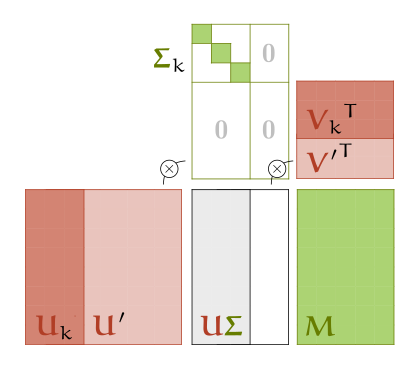
\includegraphics[width=0.8\textwidth]{./images/pca-4/svd-split.pdf}
  }
\end{figure}

\[
  \gc{\mbM} =
  \left [ \rc{\mbU}_k \; \rc{\mbU}'\right ]
  \left [ \begin{matrix}
  \gc{\Sigma}_k & \kc{\mathbf 0} \\
  \kc{\mathbf 0} & \kc{\mathbf 0} \\
  \end{matrix}\right ]
  \left [\rc{\mbV}_k \;\rc{\mbV}'\right]
 \]


%<figure class="narrow centering">
%<img src="/images/pca-4/svd-split.svg" class="three-quarters">
%<figcaption>\[ \gc{\M} =
% \left [ \rc{\U}_k \; \rc{\U}'\right ]
%\left [ \begin{array}
%~\gc{\Sigma}_k & \kc{\mathbf 0} \\
%\kc{\mathbf 0} & \kc{\mathbf 0} \\
%\end{array}\right ]
%\left [\rc{\V}_k \;\rc{\V}'\right]\] &nbsp;
%</figcaption>
%</figure>

We can now prove what we want---that \(\rc{\mbU}'\), \(\rc{\mbV}'\), and the zeroes around \(\gc{\Sig}_k\) aren't necessary to decompose \(\gc{\mbM}\)---simply by a small number of rewriting steps. To do this, it's useful to know how matrix multiplication distributes over this concatenation operator \(\left [\;\right ]\). It depends on whether the ``split'' in the matrix is parallel to the dimension we match to multiply or orthogonal to it.

If the split is parallel, as in the multiplication \(\left [ \begin{matrix}\mbA\\ \mbB \end{matrix}\right] \mbC\), the result is another concatenated matrix, but with each submatrix multiplied by \(\mbC\):

\[\left [ \begin{matrix} \mbA \\ \mbB \end{matrix}\right] \mbC = \left [ \begin{matrix}~\mbA\mbC\\ \mbB\mbC \end{matrix} \right]
\]

If the split is orthogonal, as in the multiplication \(\left [\mbA \;\mbB \right]\,\mbC\),  we must split the other matrix \(\mbC\) into submatrices \(\mbC_1\), \(\mbC_2\) to match, and the result is the sum:

\[\left [\,\mbA \;\mbB \,\right]\,\mbC = \mbA\mbC_1 + \mbB\mbC_2 \p\]

With these two rules, we can take the full SVD, and simply distribute the matrix multiplications out over the various concatenations.

\begin{align*} 
\gc{\mbM} &= \rc{\mbU}\gc{\Sig}\rc{\mbV}^T \\
&=  \left [ \rc{\mbU}_k \; \rc{\mbU}'\right ]
\left [ \begin{matrix}
\gc{\Sigma}_k & \kc{\mathbf 0} \\
\kc{\mathbf 0} & \kc{\mathbf 0} \\
\end{matrix}\right ]
\rc{\mbV}^T\\
&=  \rc{\mbU}_k 
\left [ \begin{matrix}
~\gc{\Sigma}_k & \kc{\mathbf 0} \\
\end{matrix}\right ]
\rc{\mbV}^T + \kc{\mbU'\left [ \begin{matrix}
~ \mathbf 0 &  \mathbf 0 \\
\end{matrix}\right ] \mbV^T}\\ 
&=  \rc{\mbU}_k 
\left [ \begin{matrix}
~\gc{\Sigma}_k & \kc{\mathbf 0}
\end{matrix}\right ]
\left [\rc{\mbV}_k^T \;\rc{\mbV}'^T\right]\\
&=  \rc{\mbU}_k 
\gc{\Sigma}_k
\rc{\mbV}_k^T + \kc{\mbU_k{\mathbf 0} \mbV'^T} \\
&=  \rc{\mbU}_k 
\gc{\Sigma}_k
\rc{\mbV}_k^T
\end{align*}
\hfill\qed
\end{proof}


\index{Pre-image}
\begin{theorem}
 The pre-image of a point in a column space is orthogonal to the column space.
\end{theorem}
\begin{proof}

Let \(\gc{\mbM}\mbx = \gc{\mbM}\mby\), let \(\mbz \in \text{col }\gc{\mbM}\) and let \(\gc{\mbM} = \left[\,\gc{\mbm}_1 \ldots \gc{\mbm}_m\,\right]\). Then, for some \(z'_1 \ldots z'_m\) we can write \(\mbz = z'_1\gc{\mbm}_1 + \ldots + \mbz'_m\gc{\mbm}_m\). Thus,


\begin{align*}
\mbz^T(\mbx - \mby) &= (z'_1\gc{\mbm}_1 + \ldots + \mbz'_m\gc{\mbm}_m)^T(\mbx - \mby) \\
&= (z'_1\gc{\mbm}_1x_1 + \ldots + \mbz'_m\gc{\mbm}_mx_m) - (z'_1\gc{\mbm}_1y_1 + \ldots + \mbz'_m\gc{\mbm}_my_m) \\
&= \mbz'\gc{\mbM}\mbx - \mbz'\gc{\mbM}\mby = 0 \p
\end{align*}

This tells us that the difference between any two vectors in the pre-image of a point is orthogonal to any vector in the column space of \(\gc{\mbM}\), so the two are orthogonal.\hfill\qed
\end{proof}

\section[For Chapter 5]{For Chapter~\ref{chapter:algorithms}}

%### Uniqueness of the QR decomposition

\index{QR decomposition!uniqueness}

In our discussion, we occasionally make the leap from showing that we can derive \emph{a} QR decomposition to taking that to be \emph{the} QR decomposition. Under the right conditions, this is justified: if \(\gc{\mbM}\) is full rank, a QR decomposition with only positive elements on the diagonal of \(\mbR\) is unique.

That is, for any QR decomposition, we can always create another valid QR decomposition by flipping the sign on one of the columns of \(\rc{\mbQ}\) and changing the sign of the corresponding row of \(\mbR\). But up to the variations we can create by these sign changes, the decomposition is unique.

This trick can also be used to show that such a QR decomposition always exists. Just take any QR decomposition, and flip the sign for any row of \(\mbR\) where the diagonal element is negative. We'll call this a \emph{positive QR decomposition}.

\index{QR decomposition!positive}

\begin{theorem}[Uniqueness of the positive QR decomposition] For an \(n \times m\) matrix \(\gc{\mbM}\) with linearly independent columns, the positive QR decomposition \(\rc{\mbQ}\mbR = \gc{\mbM}\) is unique.
\end{theorem}
\begin{proof}
Let \(\rc{\mbQ}\), \(\mbR\) and \(\rc{\mbP}\), \(\mbB\) be two positive QR decompositions of \(\gc{\mbM}\).

This suggests that \(\rc{\mbQ}\mbR = \rc{\mbP}\mbB\) and thus \(\rc{\mbP}^T\rc{\mbQ} = \mbB\mbR^{-1}\).

\begin{aside}
Note that \(\mbR\) is invertible because \(\gc{\mbM}\)'s columns are linearly independent. A triangular matrix is invertible if and only if its diagonal is nonzero everywhere (the determinant is the diagonal product), and a diagonal element in \(\mbR\) is zero if we can express one column of \(\gc{\mbM}\) as a linear combination of the other vectors.

Note also that while \(\rc{\mbP}\) isn't square, so not invertible, the fact that its columns are mutually orthogonal unit vectors still gives us \(\rc{\mbP}^T\rc{\mbP} = \mbI\), allowing us to move \(\rc{\mbP}\) to the left side of the equation.
\end{aside}

Now, we can conclude the following:
\begin{enumerate}
\item The inverse of \(\mbR\) must be upper triangular as well. By definition \(\mbR\mbR^{-1} = \mbI\), and having a non-zero element below the diagonal on \(\mbR^{-1}\) would create a non-zero element below the diagonal in \(\mbR\mbR^{-1}\) (note that all elements of \(\mbR\) must be non-zero).
\item The product of two upper triangular matrices is itself upper triangular. This follows from the fact that element \(i, j\) of the multiplication \(\mbA\mbB\) is the dot product of the \(i\)-th row of \(\mbA\) and the \(j\)-th column of \(\mbB\). If both are upper triangular, then all elements up to \(i\) are zero in this row of \(\mbA\) and all elements after \(j\) are zero in the column of \(\mbB\). If we are below the diagonal, them \(i>j\), so every term in the dot product is zero.
\item Since \(\mbR\) has a positive diagonal, so does its inverse. We can see from a matrix multiplication diagram that the elements that create the diagonal in the product are only the diagonal elements of \(\mbR^{-1}\), the rest are multiplied by zeroes. Since the resulting diagonal elements need to be zero, the diagonal elements of \(\mbR^{-1}\) must be the inverses of those of \(\mbR\). So if the diagonal elements of \(\mbR\) are positive, so are those of \(\mbR^{-1}\). By similar logic, we can see that \(\mbB\mbR^{-1}\) has a positive diagonal.
\item \(\rc{\mbP}^T\rc{\mbQ}\) is an orthogonal matrix. Note that \(\text{col } \mbP = \text{col }\rc{\mbQ}\), so we can express the columns of \(\rc{\mbQ}\) as linear combinations of those of \(\rc{\mbP}\), or, for some \(\rc{\mbS}\) we have \(\rc{\mbP}\rc{\mbS} = \rc{\mbQ}\). Multiplying a vector by a matrix with orthonormal columns preserves lengths and dot products, so the columns of \(\rc{\mbS}\) must be orthonormal too. Since \(\rc{\mbS}\) is square, it's orthogonal. Finally \(\rc{\mbP}\rc{\mbS} = \rc{\mbQ}\) implies \(\rc{\mbS} = \rc{\mbP}^T\rc{\mbQ}\).
\end{enumerate}


In conclusion, \(\rc{\mbP}^T\rc{\mbQ} = \mbB\mbR^{-1}\) tells us two things. From the left hand side, that this is an orthogonal matrix, and from the right hand side, that it is upper triangular with a positive diagonal.

What does an orthogonal upper triangular matrix with a positive diagonal look like? We know that its first column must be a unit vector, with zeros everywhere except the first element. Its second vector must be orthogonal to the first, so its first element must be zero, as must everything below the diagonal to keep our matrix triangular. The only remaining nonzero element is on the diagonal, so it must be 1 to make the column a unit vector.

If we keep going like this, we see that all columns must be zero above the diagonal to keep them orthogonal to the previous columns, zero below the diagonal to keep the matrix triangular, and 1 on the diagonal to keep the column a unit vector.

\begin{aside}Note that we can't make the diagonal -1 because we've concluded that the diagonal is positive everywhere.
\end{aside}

In short, we have shown that \(\rc{\mbP}^T\rc{\mbQ} = \mbB\mbR^{-1} = \mbI\). That means that \(\rc{\mbP}^T\) is the inverse of \(\rc{\mbQ}\) and \(\mbR^{-1}\) is the inverse of \(\mbB\). Since the inverse is unique, \(\rc{\mbP} = \rc{\mbQ}\) and \(\mbR = \mbB\).\hfill\qed
\end{proof}
